\quad \quad You may have noticed in the previous exercise that question 2 is particularly \\ interesting. There is a restriction on the domain of \(h(x)\). Why is that? This is what this chapter is all about. However, before we explain that, I will go over some definitions of properties of functions. Firstly, we have \textit{injection}. 
\begin{definition}
  An injective function, \(f\), or a \textit{one-to-one} function, is a function such that every distinct output of the function corresponds to only \textit{one} distinct input, that is:  
  \marginnote{\footnotesize \textit{By contraposition, \(x_1 \neq x_2\) \\ implies \(f(x_1) \neq f(x_2)\).}}
  \begin{equation*}
    f(x_1) = f(x_2) \text{\, implies \,} x_1 = x_2 
  \end{equation*}
\end{definition}
\newpage
Of course, this explanation might not have been very clear. Here is a visualisation:
\begin{figure}[h]
\centering
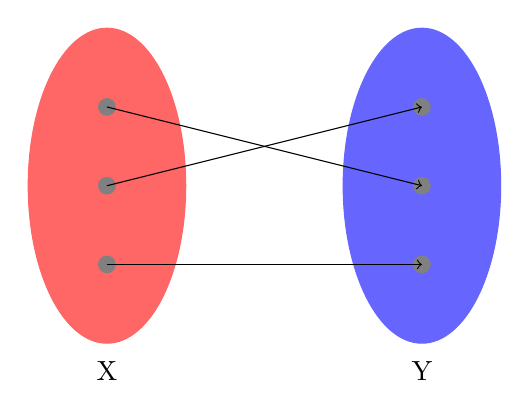
\begin{tikzpicture}
  \filldraw [red!60] (0,0) ellipse (1cm and 2cm) node[below, yshift=-60, color=black]{X}; 
  \filldraw [blue!60] (4,0) ellipse (1cm and 2cm) node[below, yshift=-60, color=black]{Y};
  \filldraw [gray] (0,1) circle (3pt);
  \filldraw [gray] (0,0) circle (3pt);
  \filldraw [gray] (0,-1) circle (3pt);
  \filldraw [gray] (4,1) circle (3pt);
  \filldraw [gray] (4,0) circle (3pt);
  \filldraw [gray] (4,-1) circle (3pt);
  \draw[->, black] (0,1) -- (4,0);
  \draw[->, black] (0,0) -- (4,1);
  \draw[->, black] (0,-1) -- (4,-1);
\end{tikzpicture} 
\caption{Illustration of an injective function with domain \(X\) and range \(Y\).}
\label{inj}
\end{figure}


As you can see in \Cref{inj}, every output in \(Y\) of the function is associated with only one input in \(X\), hence the function is \textit{injective}. To prove that a function \(f\) is injective, you can either show that if \(x_1 \neq x_2\), then \(f(x_1) \neq f(x_2)\), or if \(f(x_1) = f(x_2)\), then \(x_1 = x_2\).
\begin{figure}[h]
\centering
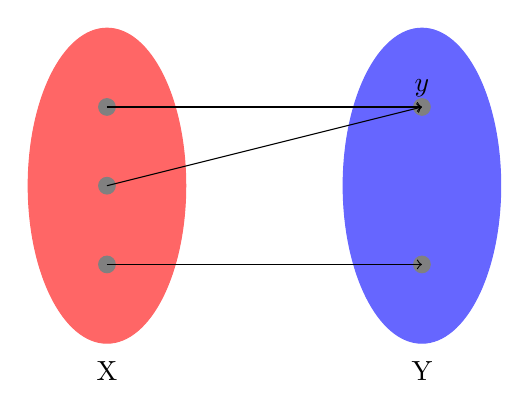
\begin{tikzpicture}
  \filldraw [red!60] (0,0) ellipse (1cm and 2cm) node[below, yshift=-60, color=black]{X}; 
  \filldraw [blue!60] (4,0) ellipse (1cm and 2cm) node[below, yshift=-60, color=black]{Y};
  \filldraw [gray] (0,1) circle (3pt);
  \filldraw [gray] (0,0) circle (3pt);
  \filldraw [gray] (0,-1) circle (3pt);
  \filldraw [gray] (4,1) circle (3pt) node[above, color=black]{\(y\)};
  \filldraw [gray] (4,-1) circle (3pt);
  \draw[->, black] (0,1) -- (4,1);
  \draw[->, black] (0,0) -- (4,1);
  \draw[->, black] (0,-1) -- (4,-1);
\end{tikzpicture} 
\caption{Illustration of a non-injective function with domain \(X\) and range \(Y\).}
\label{non_inj}
\end{figure}


Here, the function is \textit{not} injective. As you can see in \Cref{non_inj}, the output \(y\) is associated with more than one input in \(X\). With this in mind, it is time to talk about \textit{surjection}. 
\begin{definition}
  A surjective function \(f\) is a function such that for every output \(y\), there exists at least one input \(x\) such that \(f(x)=y\). 
\end{definition}


From \Cref{inj} and \Cref{non_inj}, both functions are surjective as every output is associated with at least one input. Do take note that it does not matter how many inputs associate to one output, as long every output is associated with at least one input, the function is surjective. To prove that a function is surjective, you must show that there exists an element in the domain of the function for any arbitrary output in the range.
\newpage
\begin{figure}[h]
\centering
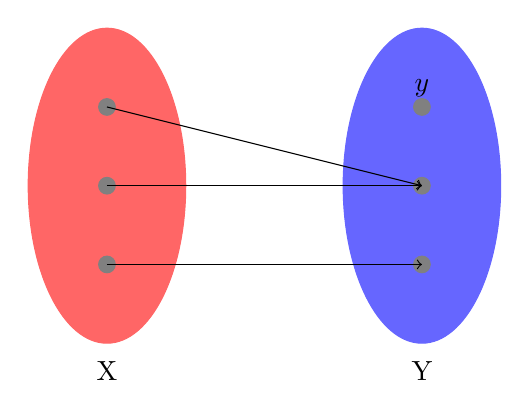
\begin{tikzpicture}
  \filldraw [red!60] (0,0) ellipse (1cm and 2cm) node[below, yshift=-60, color=black]{X}; 
  \filldraw [blue!60] (4,0) ellipse (1cm and 2cm) node[below, yshift=-60, color=black]{Y};
  \filldraw [gray] (0,1) circle (3pt);
  \filldraw [gray] (0,0) circle (3pt);
  \filldraw [gray] (0,-1) circle (3pt);
  \filldraw [gray] (4,1) circle (3pt) node[above, color=black]{\(y\)};
  \filldraw [gray] (4,0) circle (3pt);
  \filldraw [gray] (4,-1) circle (3pt);
  \draw[->, black] (0,1) -- (4,0);
  \draw[->, black] (0,0) -- (4,0);
  \draw[->, black] (0,-1) -- (4,-1);
\end{tikzpicture} 
\caption{Illustration of non-surjective function with domain \(X\) and range \(Y\).}
\label{nsurj}
\end{figure}


From \Cref{nsurj}, we can see that \(y\) has no input associated with it. As a result, the function here is not surjective. Lastly, \textit{bijective} functions can't be any easier.
\begin{definition}
  A bijective function is a function that is both injective and surjective. 
\end{definition}


However, bijective functions have a superpower. A function is only bijective \textit{if and only if} it has an inverse. \marginnote{\footnotesize \textit{P iff Q, or "P if or only if Q", means that "if P then Q" and "if Q then P".}}
\begin{theorem}
  A function, \(f:A \to B\), has an inverse if and only if it is bijection.
\end{theorem}
\begin{proof}
  To begin such proofs where there is a "if and only if" clause, we will prove both cases separately. First, we claim that if the function has an inverse, then it is bijective.
\end{proof}
\begin{lemma}
  If a function, \(f: A \to B\), has an inverse, then it is bijective. 
\end{lemma}
\begin{proof}
  Suppose \(f^{-1}\) is the inverse of \(f\). Notice that \(f^{-1}(f(x))\) is injective as it is simply \(f(x)=x\). Suppose \(a, a^\prime \in A\) and \(f(a)=f(a^\prime)\), then \(f^{-1}(f(a))=f^{-1}(f(a^\prime)))\). Notice that by injectivity of \(f^{-1}(f(x))\), \(a=a^\prime\). Hence, \(f\) is injective. Then, suppose \(b \in B\), we wish to show that the function is surjective. Notice that \(f(f^{-1}(x))\) is surjective as again, it is the identity function.
\end{proof}
